\documentclass[../main.tex]{subfiles}
\usepackage{array}
\usepackage{booktabs}
\usepackage{url}

\begin{document}

\section{Modell B: Tagesaktuelle Risikoberechnung}
\vspace{-0.5cm}
\noindent\textit{\small Verfasst von Kilian}
\vspace{0.5cm}

\subsection{Daten}

\subsubsection{Datenübersicht}
Die Modellstruktur integriert drei Datenkategorien: (i) meteorologische und hydrologische Parameter, (ii) DEM-basierte morphometrische Parameter sowie (iii) ein verifiziertes Erdrutsch-Ereigniskataster als Ground Truth. Alle Datensätze wurden in ein einheitliches Koordinaten- und Rasterbezugssystem überführt und in physikalisch konsistente Einheiten transformiert. \\

Wie bereits in Modell A beschrieben, basieren die Ground-Truth-Ereignisdaten auf dem Erdrutschkataster des IFFI-Projekts \autocite{trigilaQualityAssessmentItalian2010}, das über das Geoportal der Autonomen Provinz Bozen bezogen wurde.\\

Sämtliche atmosphärischen und hydrologischen Variablen entstammen dem Datensatz ,,ERA5 Hourly data on single levels from 1940 to present`` des Copernicus Climate Data Store \autocite{ERA5HourlyData}. Die Daten liegen in stündlicher Auflösung vor und werden im Modell auf Tageswerte aggregiert, um eine konsistente tägliche Auflösung für den Zeitraum 2015--2025 zu erzeugen. Topographische und morphometrische Parameter (Slope, Aspect, Krümmung, TWI) wurden aus dem Digitalen Geländemodell Copernicus GLO-30 abgeleitet \autocite{opentopographyCopernicusGLO90Digital2021} sowie ergänzend vom Geodatenportal Südtirol der Autonomen Provinz Bozen (2024) bezogen.

\begin{table}[ht]
    \small
    \centering
    \caption{Übersicht der verwendeten Daten, Prädiktoren und Einheiten}
    \vspace{0.5cm}
    \renewcommand{\arraystretch}{1.25}
    \begin{tabular}{
        >{\centering\arraybackslash}m{3.5cm}
        >{\centering\arraybackslash}m{3.2cm}
        >{\centering\arraybackslash}m{3.0cm}
        >{\centering\arraybackslash}m{2.5cm}
        >{\centering\arraybackslash}m{3.0cm}
        }
        \toprule
        \textbf{Prädiktor}       & \textbf{Quelle / Produkt} & \textbf{Natives Format}          & \textbf{Native Einheit} & \textbf{Finale Einheit / Form} \\
        \midrule
        Temperatur (t2m)         & ERA5 Single Levels$^{*1}$ & NetCDF (Instant, 0{,}25$^\circ$) & Kelvin (K)              & Celsius ($^\circ$C)            \\
        Niederschlag (tp)        & ERA5 Single Levels$^{*1}$ & NetCDF (Accum, 0{,}25$^\circ$)   & Meter (m)               & Millimeter (mm)                \\
        Schneefall (sf)$^{*4}$   & ERA5 Single Levels$^{*1}$ & NetCDF (Accum, 0{,}25$^\circ$)   & Meter (m)               & Millimeter (mm)                \\
        Schneehöhe (sd)          & ERA5 Single Levels$^{*1}$ & NetCDF (Instant, 0{,}25$^\circ$) & Meter (m)               & Millimeter (mm)                \\
        Bodenfeuchte (swvl1--4)  & ERA5 Single Levels$^{*1}$ & NetCDF (Instant, 0{,}25$^\circ$) & m$^3$/m$^3$             & m$^3$/m$^3$                    \\
        Hangneigung (Slope)      & Slope$^{*2}$              & GeoTIFF (10 m)                   & Grad ($^\circ$)         & Grad ($^\circ$)                \\
        Plan-/Profilkrümmung     & DEM$^{*3}$                & GeoTIFF (30 m)                   & Höhe (m)                & Krümmung (m$^{-1}$)            \\
        Exposition (Aspect)      & DEM$^{*3}$                & GeoTIFF (30 m)                   & Grad (0--360$^\circ$)   & Trig. Skalar ($-1 \dots +1$)   \\
        Feuchtigkeitsindex (TWI) & DEM (abgeleitet)$^{*3}$   & GeoTIFF (30 m)                   & --                      & Skalar (TWI)                   \\
        \bottomrule
    \end{tabular}

    \vspace{0.3cm}
    \footnotesize
    $^{*1}$ Copernicus Climate Change Service (C3S): ERA5 Single Levels Reanalysis \autocite{ERA5HourlyData}.\\
    $^{*2}$ Autonome Provinz Bozen – Südtirol (2024). \textit{Geobrowser Südtirol – Mapview}.\\
    $^{*3}$ Digitales Höhenmodell, \autocite{opentopographyCopernicusGLO90Digital2021}.\\
    $^{*4}$ Schneefall wurde in Vorstudien geprüft, jedoch im finalen Feature-Set verworfen.
\end{table}

Die ERA5-Daten wurden aufgrund ihrer konsistenten Verfügbarkeit, offenen Zugänglichkeit sowie des moderaten Speicher- und Rechenaufwands gegenüber höherdimensionalen Reanalyseprodukten ausgewählt.
Aufgrund des begrenzten Projektzeitraums verzichtet das Modell auf speicherintensive regionale Reanalysemodelle.
Die gewählte Datenbasis betont zudem die Bedeutung frei verfügbarer Daten für Transparenz und methodische Reproduzierbarkeit.

\subsubsection{Ereigniskataster Südtirol}
Nach der Datenbereinigung umfasste der Modell-Datensatz 812 Stichproben, bestehend aus 112 verifizierten Erdrutschereignissen und 500 zufällig generierten Negativbeispielen (Pseudo-Absences), die keine räumliche Überschneidung mit den Ereignispunkten aufweisen.
Die Generierung dieser Punkte erfolgte (analog zur Methodik in Modell A) zur effektiven Abbildung der Hintergrundverteilung. Jeder Datensatz ist durch Koordinaten, Datum sowie die Binärlabels 1 (Ereignis) und 0 (kein Ereignis) definiert \autocite{trigilaQualityAssessmentItalian2010a}. \\

Zur Modelloptimierung wurden zusätzlich 200 Negativpunkte explizit an steilen Hängen (Hangneigung $\ge 15^\circ$ bis max.\ $90^\circ$) generiert.
Diese Steilhang-Negative adressieren eine strukturelle Verzerrung der Trainingsdaten: Da die rein zufällig gesetzten Bezugspunkte teils im flachen Gelände liegen, könnte der Klassifikator andernfalls die triviale Regel ,,Steilheit $\Rightarrow$ Ereignis`` erlernen. Durch die in steilen Lagen forcierten Negativpunkte wird die Klassentrennung für Gebiete mit hoher Reliefenergie erzwungen, was das Modell zwingt, vorwiegend hydrologische Zustände als Differenzierungsmerkmale abzuwägen \autocites{stegerChallengeTrivialAreas2017a,stegerCorrelationDoesNot2021}.

\subsubsection{Problem der ERA5 Niederschlagsvariable tp}
Die Variable Niederschlag (\texttt{tp}) der ERA5-Reanalyse lag im Snapshot-Format (\texttt{stepType: accum}) vor und erfasste nicht die korrekte 24-h-Akkumulation, sondern lediglich den Wert der letzten Stunde vor Tageswechsel. Daraus resultierten unplausibel niedrige Tages- und Mehrtages-Niederschlagssummen, woraufhin diese Prädiktoren in ihrer Bedeutung für das Random-Forest Ensemble abgewertet wurden. \\

Als einheitlicher proxybasierter Ersatz in den Modellberechnungen diente die tiefe Bodenfeuchte (\texttt{Soil\_L4}, 100--289\,cm). Sie bildet das Maß der langfristigen hydrologischen Vorsättigung besser ab und kompensiert die lückenhafte Niederschlagsakkumulation.

\subsubsection{Ausschluss optischer Sentinel-2-Indizes}
Im Vorfeld wurden Spektral-Indizes aus optischen Sentinel-2 L2A Daten (wie NDVI, NDWI, BSI) \autocite{Sentinel2L2A} als eventuelle triggernahe Oberflächenindikatoren geprüft. Für die alpine Anwendbarkeit erwies sich deren Integration als unzureichend, da die Starkniederschlagsphasen vor Erdrutschen zumeist mit dichter Bewölkung einhergehen. Die resultierenden Satellitenbilder waren in entscheidenden Zeitfenstern wolkenverdeckt oder wiesen Schattenartefakte auf. \\

Großräumige und tagesaktuelle Szenenmosaike per STAC (SpatioTemporal Asset Catalog) \autocite{STACSpatioTemporalAsset} und Xarray \autocite{XarrayNDLabeled} verursachten Speicher- und Rechenaufwand, was eine operationelle Anwendung verhinderte.
Da die Integration stattdessen die Varianz drastisch erhöhte und inkohärente Prädiktorsignale erzeugte, kam es zu einem Einbruch der Modellqualität.
Entsprechend wurden Sentinel-2-Indizes aus dem finalen Variablen-Set vollständig ausgeschlossen, obgleich die zukünftige Kombination mit radarbasierter Change-Detection perspektivisch ein wertvolles Entwicklungsfeld darstellt.

\subsection{Methodik}

\subsubsection{Referenzgitter}

Die räumliche Modellierung der Risikoberechnung erfolgt auf einem einheitlichen Referenzgitter mit einer Auflösung von $500 \times 500$\,m im Koordinatensystem ETRS89 / UTM Zone 32N (EPSG:25832).
Dieses Referenzgitter bildet die verbindliche räumliche Bezugsbasis aller Modellvariablen. Morphometrische und hydrologische Parameter werden zunächst im nativen Format der jeweiligen Reliefdaten berechnet. Anschließend erfolgt die Aggregation sämtlicher Parameter auf das 500-m-Referenzgitter durch flächenbasierte Mittelwertbildung. Jede 500-m Zelle enthält somit sowohl einen räumlich statischen topographischen Kennwert als auch die zugehörigen dynamischen meteorologischen und bildet die konsistente räumliche und zeitliche Integration des Modells.
\subsection{Hangneigung, Profil- und Plankrümmung}

Während die Hangneigung als prägender Auslöser bereits in Modell A
erörtert wurde, sind für dieses Modell Profil- und Plankrümmung zusätzlich essenziell.
Krümmungsformen bestimmen, wo Wasser beschleunigt, gebremst, lateral gebündelt oder verteilt wird. Gefahrenzonen für Erdrutsche können aus diesen räumlichen Eigenschaften resultieren \autocite{ohlmacherPlanCurvatureLandslide2007}.
Die Plan- und Profilkrümmung werden nach \textcite{zevenbergenProfileCurvature1987} über eine lokale quadratische Oberflächenapproximation in einem $3 \times 3$-Rasterfenster berechnet.
Grundlage sind die ersten Ableitungen


\[
    p = \frac{\partial z}{\partial x}\qquad
    q = \frac{\partial z}{\partial y}
\]


sowie die zweiten Ableitungen



\[
    r = \frac{\partial^2 z}{\partial x^2} \qquad
    s = \frac{\partial^2 z}{\partial x \partial y} \qquad
    t = \frac{\partial^2 z}{\partial y^2}
\]


Dabei bezeichnet \( z \) die Geländehöhe  \([\mathrm{m}]\),  \( x \) und \( y \) die horizontalen Koordinaten, und  \( p \) und \( q \)  die Steigungskomponenten (dimensionslos, \(\mathrm{m/m}\))  und \( r, s, t \)  die Krümmungskomponenten mit der Einheit \([\mathrm{m^{-1}}]\).


Die normierten Krümmungsformeln lauten


\[
    \mathrm{ProC} =
    -2 \cdot
    \frac{r p^2 + 2 s p q + t q^2}{p^2 + q^2}
\]

und

\[
    \mathrm{PlnC} =
    2 \cdot
    \frac{r q^2 - 2 s p q + t p^2}{p^2 + q^2}.
\]

Beide Größen besitzen die Einheit \([\mathrm{m^{-1}}]\), da die zweiten Ableitungen \([\mathrm{m^{-1}}]\), sind und der Nenner  \( p^2 + q^2 \)  dimensionslos ist.


Die Profilkrümmung charakterisiert die Krümmung der Oberfläche entlang der Falllinie und beschreibt die Änderung der Neigung in Richtung des maximalen Gefälles.

\[
    \mathrm{ProC} < 0
\]

kennzeichnet eine konkave Form mit tendenzieller Abflussbremsung und Akkumulation, während

\[
    \mathrm{ProC} > 0
\]

eine konvexe Form mit Abflussbeschleunigung und erhöhter erosiver Wirkung beschreibt.

Die Plankrümmung  beschreibt die Krümmung quer zur Falllinie und quantifiziert laterale Konvergenz bzw. Divergenz.

\[
    \mathrm{PlnC} < 0
\]

steht für konvergente Formen (Rinnen, Hohlformen) mit lateraler Wasserzusammenführung,

\[
    \mathrm{PlnC} > 0
\]
für divergente Formen (Rücken, Kämme) mit Wasserverteilung.


\begin{figure}[htbp]
    \centering
    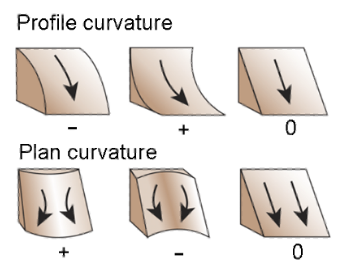
\includegraphics[width=0.45\textwidth]{../img/profilcurvature.png}
    \caption{Visuelle Darstellung der Werteverhalten, Quelle: \autocite{zaragoziDataDrivenStudy2013}}
    \label{fig:curvature_distribution}
\end{figure}


\subsection{3.3 Exposition}



Die Exposition (Hangausrichtung, engl. Aspect) bezeichnet den Azimut der Falllinie, also die Richtung des maximalen Gefälles eines Geländepunktes. Sie bestimmt die Orientierung des Oberflächenabflusses und beeinflusst über strahlungsabhängige Prozesse die räumliche Verteilung von Energieeintrag, Verdunstung und Bodenfeuchte auf einem Hang \autocite[54-56]{wilsonTerrainAnalysisPrinciples2000}. Ebenfalls kann dies Einfluss auf Gefahrenzonen für Erdrutsche hinweisen \autocite{capitaniSlopeAspectPredisposing2013}. Die Exposition wird aus den Gradientenkomponenten des DEM berechnet. Aus den ersten Ableitungen nach \textcite{zevenbergenQuantitativeAnalysisLand1987}


\[
    p = \frac{\partial z}{\partial x}\qquad
    q = \frac{\partial z}{\partial y}
\]

ergibt sich der Azimut der Falllinie als

\[
    \mathrm{aspect} = \operatorname{atan2}(-p,\, q).
\]


Die Verwendung der zweistelligen Arkustangensfunktion
$\operatorname{atan2}$ gewährleistet eine Quadrantenzuordnung im Bereich (0°, 360°) \autocite{zevenbergenQuantitativeAnalysisLand1987}.

Das Minuszeichen vor p ergibt sich aus der Konvention, dass die Exposition in Richtung des steilsten Gefälles und nicht des Anstiegs definiert ist. In der Winkelrepräsentation entsteht zwischen 0° und 360° eine künstliche Diskontinuität, die in maschinellen Lernverfahren als numerischer Sprung wirken kann. Zur Auflösung dieser Zirkularität wird die Exposition trigonometrisch in zwei orthogonale Komponenten transformiert.



\[
    \mathrm{Aspect}_{North} = -\cos(\mathrm{aspect})
    \qquad
    \mathrm{Aspect}_{East} = \sin(\mathrm{aspect}).
\]



Dadurch entstehen kontinuierliche Skalarwerte im Bereich (-1, +1), welche die Nord- bzw. Ost-Komponente der Falllinie beschreiben und keine Winkel-Diskontinuität mehr aufweisen.\autocite{fisherStatisticalAnalysisCircular1993}.



\subsection{Modifizierter Topographic Wetness Index (TWI)}


Zur Abbildung topographisch begünstigter Wasserakkumulation wird ein modifizierter Topographic Wetness Index (TWI) implementiert. Der klassische TWI definiert sich als


\[
    \mathrm{TWI} = \ln\!\left(\frac{a}{\tan \beta}\right)
\]


wobei das spezifische Einzugsgebiet $\alpha$ (Upslope Contributing Area per unit contour length) und $\beta$ die lokale Hangneigung ist \autocite{bevenPhysicallyBasedVariable1979a}. Die explizite Berechnung eines hydrologisch konsistenten Einzugsgebiets ist im vorliegenden Modellansatz mit anschließender Aggregation auf 500 m jedoch methodisch aufwendig und stark parameterabhängig.

Stattdessen wird ein geometrischer Proxy verwendet, der laterale Konvergenz über die Plan-Krümmung abbildet \autocite{zevenbergenQuantitativeAnalysisLand1987}.


Der implementierte Index lautet:

\[
    twi = \ln\left(\frac{catchment\_proxy}{\tan(slope_{rad})}\right)
\]

mit

\[
    \mathrm{catchment\_proxy}
    =
    \max\!\left(
    0.1,\;
    1.0 + \mathrm{plan\_c} \cdot 100.0
    \right)
\]

Der Wert 1,0 steht für neutrales, planes Gelände. Positive Plankrümmung erhöht, negative reduziert den catchment proxy. Aufgrund der geringen numerischen Größenordnung der Krümmung wird ein Faktor 100 zur Skalierung verwendet. Die Untergrenze von 0,1 stellt die Positivität des Logarithmusarguments sicher. Es handelt sich um einen vereinfachten Proxy zur Approximation lateraler Wasserakkumulation ohne explizite Flussrichtungsberechnung.


\subsection{ERA5-Reanalyse und orographische Korrekturen}

ERA5 Singel Levels liegen nativ in einer räumlichen Auflösung von etwa 0,25° (28 km) vor \autocite{ERA5HourlyData}. Um die Skaleninkonsistenz zwischen einer homogenen ERA5 0,25° Zell und einer 500-m Raster Zelle physikalisch zu reduzieren, werden orographische Korrekturen implementiert. Dazu wird eine ERA5-Referenzorographie abgeleitet und die Höhendifferenz \(\Delta h\) zwischen 500-m Zelle und ERA5-Referenzhöhe gebildet.

Die 2-m-Temperatur wird zunächst von Kelvin nach Celsius transformiert

\[T_{^\circ\mathrm{C}} = T_{\mathrm{K}} - 273{,}15\]

Anschließend erfolgt eine höhenabhängige Anpassung über den klimatologischen Standardgradienten

\[T_{\mathrm{corr}} = T_{^\circ\mathrm{C}} + (-0{,}0065)\, \Delta h
\]

Wie bei der Temperatur basiert auch der Niederschlag auf einer Auflösung von 0,25°, wodurch die Orographie geglättet ist.

Zur höhenabhängigen Differenzierung wird daher ein vertikaler Skalierungsfaktor angesetzt
\[
    \mathrm{rain\_factor} = 1 + \left(\frac{\Delta h}{100}\right)\cdot 0{,}08
\]





ntsprechend einer orographischen Niederschlagszunahme von +8 \% pro 100 Höhenmeter. Dieser Wert liegt innerhalb des in der alpinen Niederschlagsklimatologie dokumentierten Bereichs von etwa 5–10 \% pro 100 m \autocite{freiPrecipitationClimatologyAlps1998, sevrukRegionalDependencyPrecipitationAltitude1997}

\[
    Zur numerischen Stabilisierung wird der Faktor auf
    \mathrm{rain\_factor} \in [0{,}5;\,2{,}0]
\]

begrenzt.
Dadurch erhält ein Hang maximal die doppelte und in tiefen Lagen maximal die halbe Niederschlagsmenge als Proxy.

Die Skalierungsfaktoren fungieren als heuristische Annahme zur partiellen Kompensation der Homogenisierung innerhalb der ERA5-Reanalyse und stellt keine direkte Ableitung aus lokalen Messreihen des Unterschungsgebietes dar.



\subsection{Feature-Set}

Das finale Feature-Set umfasst 27 Prädiktoren integriert klimatische Vorläuferfenster, Bodenfeuchte in Tiefenprofil und 7-Tage Trends sowie Geländeparameter. Interaktionsterme (z. B. Slope × Soil, TWI × Rainfall) verbinden topographische Eigenschaften mit hydrologischen Triggern, um kombinierte Risikomuster statt Einzelwerte abzubilden.



\subsection{Random-Forest Training}
Analog zu Modell A fußt die Vorhersagearchitektur auf einem in scikit-learn verankerten Random-Forest Klassifikator.

Der Gesamtdatensatz wurde in 70 \% Trainingsdaten und 30 \% Testdaten aufgeteilt. Das Modelltraining erfolgte auf dem Trainingsset unter Anwendung einer fünffachen Kreuzvalidierung (5-Fold Cross-Validation, cv=5) sowie einer Randomized-Search Suche zur Hyperparameter-Optimierung, bei der 50 zufällige Parameterkombinationen (n\_iter=50) nach dem besten Ergebnis evaluiert wurden \autocite{pedregosaScikitlearnMachineLearning2011}.

Der definierte Hyperparameterraum lautet:

\begin{lstlisting}[language=Python]
param_dist = {
    'n_estimators': [200, 500, 1000],
    'max_depth': [10, 20, None],
    'min_samples_split': [2, 5, 10],
    'min_samples_leaf': [2, 4, 8],
    'max_features': ['sqrt', 'log2', 0.2, 0.3, 0.4],
    'bootstrap': [True]
}
\end{lstlisting}



Eine zentrale Herausforderung des Datensatzes ist die Klassenimbalance. 112 verifizierte Rutschungsereignisse stehen mehreren hundert Negativbeispielen gegenüber. Ohne Gegenmaßnahme würde ein Random Forest durch bloße Dominanz der Negativklasse hohe Accuracy erzielen, jedoch kaum Ereignisse erkennen.
Daher wurde wurde wie in Model A
\[
    \texttt{class\_weight} = \text{"balanced"}
\]
verwendet.
Formal bedeutet dies, dass die Gewichtung einer Klasse \(k\) invers proportional zu ihrer Häufigkeit \(n_k\) ist:

\[
    w_k \propto \frac{1}{n_k}
\]







Die native Modellausgabe ist eine Wahrscheinlichkeit \( p \) für das Auftreten
einer Rutschung. Die binäre Klassifikation erfolgt über einen Schwellenwert \( \tau \).Die Verwendung eines festen Schwellenwerts von \( \tau = 0.50 \)
führte im vorliegenden Datensatz zu einer systematischen
Unterwarnung, da ein erheblicher Anteil tatsächlicher Ereignisse
Wahrscheinlichkeiten unterhalb von 0.50 aufwies und somit nicht als
Rutschung klassifiziert wurde (Reduktion des Recalls).

Zur datengetriebenen Bestimmung eines geeigneten Schwellenwerts wird daher
der \(F_\beta\)-Score maximiert:

\[
    F_{\beta} = (1+\beta^{2}) \cdot \frac{\mathrm{Precision}\cdot \mathrm{Recall}}{(\beta^{2}\cdot \mathrm{Precision})+\mathrm{Recall}}
\]

Der \(F_\beta\)-Score stellt ein gewichtetes harmonisches Mittel aus
Precision und Recall dar. Über den Parameter \( \beta \) wird das relative
Gewicht beider Größen gesteuert. Mit \( \beta = 0.6 \) wird Precision
stärker gewichtet als Recall, wodurch Fehlalarme stärker penalisiert
werden als einzelne verpasste Ereignisse.

Die Optimierung über das Intervall \( \tau \in [0.05,\,0.95] \)
ergab schließlich \( \tau = 0.30 \).


\subsection{Ergebnisse und Modellperformanz}
\subsubsection{Klassifikationsbericht}

Die datengetriebene Hyperparameter-Optimierung konvergierte bei folgendem Parametersatz: n\_estimators= 200, max\_depth= None, min\_samples\_split= 2, min\_samples\_leaf
= 2, max\_features= 0.3 und bootstrap= True.


Die Evaluation des 70/30 Splits erfolgt auf n = 184 Samples (150 Negative, 34 Ereignisse).
Steilhang-Negative sind aus diesem Validierungs-Set ausgeschlossen, um eine Prognose über alle Wertebereiche der topographischen und hydrologischen Parameter zu gewährleisten.
Bei dem optimierten Schwellenwert von \(\tau=0,30\) ergeben sich eine Gesamtgenauigkeit (Accuracy) von 85,87 \%, eine Ereignis-Precision von 62,50 \% und ein Ereignis-Recall von 58,82 \%.




\begin{table}[h]
    \centering
    \caption{Klassifikationsbericht für $\tau = 0.30$}
    \vspace{0.5cm}
    \begin{tabular}{lcccc}
        \toprule
        \textbf{Klasse} & \textbf{Precision} & \textbf{Recall} & \textbf{F1-Score} & \textbf{Support} \\
        \midrule
        0 (Negativ)     & 0,91               & 0,92            & 0,91              & 150              \\
        1 (Ereignis)    & 0,62               & 0,59            & 0,61              & 34               \\
        \midrule
        Accuracy        &                    &                 & 0,86              & 184              \\
        Macro Avg       & 0,77               & 0,75            & 0,76              & 184              \\
        Weighted Avg    & 0,86               & 0,86            & 0,86              & 184              \\
        \bottomrule
    \end{tabular}
\end{table}





\begin{table}[ht]
    \centering
    \caption{Konfusionsmatrix des Tests ($\tau=0.30$)}
    \vspace{0.5cm}
    \label{tab:confusion_matrix_custom_clean}
    \renewcommand{\arraystretch}{1.5}
    \begin{tabular}{|l|c|c|}
        \hline
                                        & \textbf{Actually Positive (1)} & \textbf{Actually Negative (0)} \\
        \hline
        \textbf{Predicted Positive (1)} & 20                             & 12                             \\
        \hline
        \textbf{Predicted Negative (0)} & 14                             & 138                            \\
        \hline
    \end{tabular}
\end{table}
Von den 150 real sicheren Punkten wurden 138 korrekt als risikoarm klassifiziert (True Negatives), wohingegen 12 Punkte fälschlicherweise Warnungen auslösten (False Positives). Von den 34 verifizierten Erdrutschen wurden 20 Ereignisse erfolgreich identifiziert (True Positives) und 14 übersehen (False Negatives).




\subsubsection{Feature Importance}

\textbf{Bild Feutre importance}



Die Feature-Importance-Analyse zeigt eine klare Dominanz hydrologischer und klimatischer Langzeitindikatoren. Besonders die tiefe Bodenfeuchte (Soil\_L4, 14,3 \%) sowie längerfristige Temperatur- und Niederschlagsmittel prägen die Klassifikation, was auf die zentrale Rolle der hydraulischen Vorbelastung hinweist. Die Hangneigung bleibt relevant, wirkt jedoch vor allem in Kombination mit Feuchteparametern. Statische Terrainvariablen wie Krümmung oder Exposition tragen nur marginal zur Trennschärfe bei. Insgesamt wird die Erdrutschdisposition primär durch dynamische hydrologische Zustände gesteuert, während die Morphologie eine modulierende Funktion einnimmt.


\subsubsection{Modellvisualisierung und Validierung}
Die auf dem 500-m Referenzgitter berechneten Landslide Hazard Probability Maps stellen die modellierte Erdrutsch-Disposition für einen definierten Stichtag dar. Jede Rasterzelle enthält die vom Klassifikator inferierte Ereigniswahrscheinlichkeit im Bereich von 0 bis 1, die über eine kontinuierliche Farbskala visualisiert wird. Niedrige Werte kennzeichnen stabile Bereiche (Türkis), hohe Werte markieren Zonen erhöhter Disposition (Rot). Zur Validierung werden die prognostizierten Wahrscheinlichkeiten mit den dokumentierten Ereignissen des Ereigniss-Katasters räumlich verschnitten. Historische Ereignisse dienen als Referenz, während am Zieltag aufgetretene Rutschungen gesondert hervorgehoben werden (siehe Legende). Die Modell Validierung des jeweiligen Tages wird zusätzlich über die Capture Rate bestimmt, also den Anteil der Tagesereignisse, die bei Anwendung des trainierten Schwellenwerts korrekt als positiv klassifiziert wurden.

\begin{figure}[htbp]
    \centering
    
\includegraphics[width=\textwidth]{img/landslideharadmodel2020.png}
    \caption{Berechnete Risikokarte für Erdrutsche des 08.05.2021, Südtirol}
\end{figure}

\begin{figure}[htbp]
    \centering
    
\includegraphics[width=\textwidth]{img/landslideharzadmodel202012.png}
    \caption{Berechnete Risikokarte für Erdrutsche des 12.06.2020, Südtirol}
\end{figure}


Als Vergleich der Modellauswertung dienen die Tagesberechnungen für den 08.05.2021 und den 12.06.2020. Beide Termine zeigen eine deutlich unterschiedliche Ausprägung des prognostizierten Risikos.
Der erste Betrachtungstag weist großflächig erhöhte Wahrscheinlichkeiten auf. Die an diesem Tag dokumentierten Erdrutschereignisse korrelieren räumlich mit den vom Modell ausgewiesenen Hochrisikobereichen. 94,4 \% dokumentierter Ereignisse wurden am 08.05.2021 wurden korrekt erfasst. Die erhöhte Disposition verteilt sich über mehrere zusammenhängende Zonen und spiegelt eine ausgeprägte hydrometeorologische Vorbelastung wider.
Am zweiten Beispieltag fällt das berechnete Risiko insgesamt deutlich geringer aus. Die Modellentscheidung stützt sich hier primär auf die statischen topographischen Parameter, was sich in einer stärkeren Konzentration der Wahrscheinlichkeiten entlang markanter Reliefstrukturen und Bergketten zeigt. Für diesen Tag ist ein dokumentiertes Ereignis verzeichnet, das innerhalb einer vom Modell als Risiko erhöht eingestuften Fläche liegt.
Die Gegenüberstellung verdeutlicht den Einfluss meteorologischer Parameter auf die Risikoverteilung. Bei klimatischen Extremwerten streut das Risiko großflächiger, unter durchschnittlichen Bedingungen konzentriert es sich auf morphologisch prädisponierte Bereiche. Die Gefahrenkarten sind als regionales Dispositions- und Screeninginstrument zu verstehen und liefern keine parzellenscharfen Prognosen. Hohe Wahrscheinlichkeiten treten dort auf, wo morphologische Prädisposition und aktuelle hydrometeorologische Vorbelastung zusammenwirken.

\end{document}